\documentclass{beamer}
\geometry{paperwidth=100mm,paperheight=75mm}
% \usetheme{Berkeley}
% \usetheme{Boadilla}
\usetheme{Madrid}
% \usetheme{Montpellier}
% \usetheme{Warsaw}
% \usetheme{Copenhagen}
% \usetheme{Goettingen}
% \usetheme{Hannover}
% \usetheme{PaloAlto}
% \usetheme{AnnArbor}
% \usetheme{Bergen}
% \usetheme{Marburg}
%\usecolortheme{beetle}
\setbeamertemplate{page number in head/foot}{}

\usepackage{mathtools,amsthm,amssymb,mathrsfs}
\usepackage{graphicx}
\usepackage{xcolor}
% \usepackage{enumitem}

% \usepackage[backend=biber]{biblatex}
% \addbibresource{bibliography.bib}
% \usepackage{soul}
% \usepackage{float}
% \usepackage{enumerate}
% \usepackage{multicol}
% \usepackage{tikz}
% \usetikzlibrary{matrix,arrows}
\usepackage[all]{xy}
% \usepackage{tikz-cd}
% \tikzcdset{every arrow/.append style = -{Latex[width=4pt,length=10pt]}}
\usepackage[defaultmono]{droidsansmono}
\usepackage{listings}
% \lstset{basicstyle=\xpt\droidsansmono}
% \usepackage{fontspec}
% \usepackage{setspace}
% \setmainfont{Times New Roman}
% \usepackage{derivative}
% \usepackage{fancyvrb}
% \renewcommand{\theFancyVerbLine}{\textsuperscript{\arabic{FancyVerbLine}}}
% \usepackage{multirow}
% \usepackage{dsfont}
\usepackage{indentfirst}
% \usepackage{blindtext}
\usepackage{lipsum}
\usepackage{algorithm}
\usepackage{algpseudocode}
\algtext*{EndIf}
\algtext*{EndFor}
\algtext*{EndWhile}

\definecolor{codegreen}{rgb}{0,0.6,0}
\definecolor{codegray}{rgb}{0.5,0.5,0.5}
\definecolor{codepurple}{rgb}{0.58,0,0.82}
\definecolor{backcolour}{rgb}{0.95,0.95,0.92}

\lstset{escapechar=\&,
        basicstyle=\scriptsize\droidsansmono,
        breaklines=true,
        showstringspaces=false,
        backgroundcolor=\color{backcolour}}
        % commentstyle=\color{codegreen},
        % keywordstyle=\color{blue},
        % stringstyle=\color{codepurple}}

% \DeclarePairedDelimiter{\ceil}{\lceil}{\rceil}
% \DeclarePairedDelimiter{\floor}{\lfloor}{\rfloor}
% \def\bA{\mathbb{A}}
% \def\cB{\mathcal{B}}
\def\bC{\mathbb{C}}
\def\sC{\mathsf{C}}
\def\sD{\mathsf{D}}
\def\sE{\mathsf{E}}
\def\bF{\mathbb{F}}
\def\cF{\mathcal{F}}
\def\cG{\mathcal{G}}
% \def\bH{\mathbb{H}}
% \def\bI{\mathbb{I}}
% \def\cL{\mathcal{L}}
% \def\cM{\mathcal{M}}
\def\bN{\mathbb{N}}
\def\cP{\mathcal{P}}
\def\bQ{\mathbb{Q}}
\def\bR{\mathbb{R}}
\def\cT{\mathcal{T}}
\def\Hask{\mathsf{Hask}}
% \def\cU{\mathcal{U}}
% \def\bV{\mathbb{V}}
\def\bZ{\mathbb{Z}}
% \def\bk{\bk}
\def\sbs{\subseteq}
\def\sps{\supseteq}

% \DeclareMathOperator{\Aut}{Aut}
% \DeclareMathOperator{\Dim}{Dim}
% \DeclareMathOperator{\ev}{ev}
\DeclareMathOperator{\gb}{gb}
% \DeclareMathOperator{\GL}{GL}
\DeclareMathOperator{\Hom}{Hom}
\DeclareMathOperator{\id}{id}
\DeclareMathOperator{\im}{im}
\DeclareMathOperator{\lcm}{lcm}
% \DeclareMathOperator{\Mat}{Mat}
% \DeclareMathOperator{\nullsp}{null}
% \DeclareMathOperator{\range}{range}
% \DeclareMathOperator{\SL}{SL}
\DeclareMathOperator{\Span}{span}
\newcommand{\LT}{\ensuremath{\text{\sc lt}}}
\newcommand{\LM}{\ensuremath{\text{\sc lm}}}
\newcommand{\LC}{\ensuremath{\text{\sc lc}}}
\DeclareMathOperator{\multideg}{multideg}
\def\and{\text{ and }}

% \def\e{\epsilon}
% \def\d{\delta}
\def\p{\varphi}

\title{Functional Polynomial Algorithms}
\author{Thomas Meek}
\date{May 13, 2023}

% \begin{frame}{Turing Machines}
%   \Large \only<1>{Turing Machines}
%   \only<1-4>{\begin{itemize}
%     \item<2-4> Finite control (set of states)
%     \item<3-4> Head capable of reading/writing
%     \item<4> Infinite roll of tape with symbols
%   \end{itemize}}
%   \only<5->{\begin{enumerate}
%     \item<5-> read the symbol from the current cell,
%     \item<6-> print a symbol in this cell,
%     \item<7-> move one cell to the left or right,
%     \item<8-> transition into the next state.
%   \end{enumerate}}
%   \uncover<4->{\begin{figure}[b!]
%     \includegraphics[width=9cm]{images/turing_machine.png}
%     \vspace{-5mm}
%     \caption{A Turing machine with infinite tape and a finite control.
%     \cite{hopcroft79}}
%   \end{figure}}
% \end{frame}

% \uncover<2-3>{Second.}
% \uncover<3>{Third.}

\begin{document}

\frame{\titlepage}

\section{Introduction}

\begin{frame}{Linguistics}
  \center {\Large Linguistics}
  \begin{itemize}
    \item<2-> Declarative sentences
    \item<3-> Imperative sentences
    \item<4> Interrogative sentences
  \end{itemize}
\end{frame}

\begin{frame}{Linguistics}
  \center {\Large Declarative sentences}
  \begin{itemize}
    \item<2-> Steve has twelve eggs.
    \item<3> $f(x) = x^2$.
  \end{itemize}
\end{frame}

\begin{frame}{Linguistics}
  \center {\Large Imperative sentences}
  \begin{itemize}
    \item<2-> Make me an omelette. 
    \item<3> \lstinline{print("Hello world.")}
  \end{itemize}
\end{frame}

\begin{frame}{Linguistics}
  \center {\Large Interrogative sentences}
  \begin{itemize}
    \item<2-> Where are my eggs?
    \item<3-> Why is this guy talking about linguistics in a thesis defense for a mathematics degree?
  \end{itemize}
\end{frame}

\begin{frame}{Why?}
  \center {\Large Haskell}
\end{frame}

\begin{frame}{Why?}
  \begin{itemize}
    \item Procedural \uncover<4->{\hspace{5pt}\textleftarrow\hspace{5pt} Imperative} \uncover<6->{(C)}
    \item<2-> Object-oriented \uncover<4->{\hspace{5pt}\textleftarrow\hspace{5pt} Imperative} \uncover<7->{(Java)}
    \item<3-> Functional \uncover<5->{\hspace{5pt}\textleftarrow\hspace{5pt} Declarative} \uncover<8->{(Haskell)}
    \item[]<9->
    \item<9-> Math \uncover<10->{\hspace{5pt}\textleftarrow\hspace{5pt} Declarative}
  \end{itemize}
\end{frame}

\begin{frame}{Polynomials}
  \center {\Large Polynomials}
\end{frame}

\begin{frame}{Polynomials}
  \[ (x+a)^2 \uncover<2->{=_{\bF_2}x^2+a^2} \]
\end{frame}

\begin{frame}{Polynomials}
  \begin{definition}
    A \textbf{monomial} in $x_1,\dots,x_n$ is a product of the form
    \[ x_1^{\alpha_1} \cdot x_2^{\alpha_2} \cdots x_n^{\alpha_n}, \]
    where all of the exponents $\alpha_1,\dots,\alpha_n$ are nonnegative integers.
  \end{definition}
\end{frame}

\begin{frame}{Polynomials}
  \begin{definition}
    Let $\alpha = (\alpha_1,\dots,\alpha_n)$ be an $n$-tuple of nonnegative integers. Then we set
    \[ x^\alpha = x_1^{\alpha_1} \cdot x_2^{\alpha_2} \cdots x_n^{\alpha_n}. \]
  \end{definition}
\end{frame}

\begin{frame}{Polynomials}
  \begin{definition}
    A \textbf{polynomial} $f$ in the variables $x_1,\dots,x_n$ over a field $k$ is a finite linear combination (with coefficients in $k$) of monomials in $x_1,\dots,x_n$. We will write a polynomial $f$ in the form
    \[ f = \sum_\alpha a_\alpha x^\alpha,\quad a_\alpha \in k, \]
    where the sum is over a finite number of $n$-tuples $\alpha = (\alpha_1,\dots,\alpha_n)$. The set of all polynomials in $x_1,\dots,x_n$ with coefficients in $k$ is denoted $k[x_1,\dots,x_n]$.
  \end{definition}
\end{frame}

\begin{frame}{Polynomials}
  \begin{definition}
    Let $f = \sum_\alpha a_\alpha x^\alpha$ be a polynomial in $k[x_1,\dots,x_n]$.
    \begin{itemize}
      \item<2-> We call $a_\alpha$ the \textbf{coefficient} of the monomial $x^\alpha$.
      \item<3-> If $a_\alpha\ne0$, then we call $a_\alpha x^\alpha$ a \textbf{term} of $f$.
      \item<4-> The \textbf{total degree} of $f \ne 0$, denoted $\deg(f)$, is the maximum $|\alpha|$ such that the coefficient $a_\alpha$ is nonzero. The total degree of the zero polynomial is undefined.
    \end{itemize}
  \end{definition}
\end{frame}

\begin{frame}{Polynomials}
  \center {\Large Leading term}
  \uncover<2>{\[ g = x^3yz^2 + x^5 + x^2y^3z \]}
\end{frame}

\begin{frame}{Polynomials}
  \begin{definition}
    A \textbf{monomial ordering} on $k[x_1,\dots,x_n]$ is a relation $>$ on the set of monomials $x^\alpha$, $\alpha \in \bZ_{\ge0}^n$ satisfying:
    \begin{itemize}
      \item<2-> $>$ is a total ordering.
      \item<3-> If $x^\alpha > x^\beta$ and $\gamma \in \bZ_{\ge0}^n$, then $x^\alpha x^\gamma > x^\beta x^\gamma$.
      \item<4-> $>$ is a well-ordering.
    \end{itemize}
  \end{definition}
\end{frame}

\begin{frame}{Polynomials}
  \begin{theorem}
    Let $X$ be a commutative free monoid and suppose the first two conditions in the definition above are satisfied. Then the following are equivalent:
    \begin{itemize}
      \item<2-> $>$ is a well-ordering on $X$.
      \item<3-> Every strictly decreasing sequence in $X$ eventually terminates.
      \item<4-> $x^\alpha\ge1$ for all $\alpha \in \bZ_{\ge0}^n$.
    \end{itemize}
  \end{theorem}
\end{frame}

\begin{frame}{Polynomials}
  \begin{definition}[Lexicographic Order]
    Let $\alpha = (\alpha_1, \dots, \alpha_n)$ and $\beta = (\beta_1,\dots,\beta_n)$ be in $\bZ_{\ge0}^n$. We say $x^\alpha >_{Lex} x^\beta$ if the leftmost nonzero entry of the vector difference $\alpha - \beta \in \bZ^n$ is positive.
  \end{definition}
  \uncover<2>{\[ g = x^3yz^2 + x^5 + x^2y^3z \]}
\end{frame}

\begin{frame}{Polynomials}
  \begin{definition}[Graded Lex Order]
    Let $\alpha,\beta \in \bZ_{\ge0}^n$. We say $x^\alpha >_{GLex} x^\beta$ if $|\alpha| > |\beta|$ or $|\alpha|=|\beta|$ and $x^\alpha >_{Lex} x^\beta$.
  \end{definition}
  \uncover<2>{\[ g = x^3yz^2 + x^5 + x^2y^3z \]}
\end{frame}

\begin{frame}{Polynomials}
  \begin{definition}[Graded Reverse Lex Order]
    Let $\alpha,\beta \in \bZ_{\ge0}^n$. We say $x^\alpha >_{GRevLex} x^\beta$ if $|\alpha| > |\beta|$ or $|\alpha|=|\beta|$ and the rightmost nonzero entry of $\alpha - \beta \in \bZ^n$ is negative.
  \end{definition}
  \uncover<2>{\[ g = x^3yz^2 + x^5 + x^2y^3z \]}
\end{frame}

\begin{frame}{Polynomials}
  \center {\Large Ideals}
\end{frame}

\begin{frame}{Polynomials}
  \begin{definition}
    A subset $I \sbs k[x_1,\dots,x_n]$ is an \textbf{ideal} if it satisfies:
    \begin{itemize}
      \item<2-> $0 \in I$.
      \item<3-> If $f,g \in I$, then $f+g \in I$.
      \item<4-> If $f \in I$ and $h \in k[x_1,\dots,x_n]$, then $hf \in I$.
    \end{itemize}
  \end{definition}
\end{frame}

\begin{frame}{Polynomials}
  \begin{definition}
    Let $I \sbs k[x_1,\dots,x_n]$ be an ideal other than $\{0\}$, and fix a monomial ordering on $k[x_1,\dots,x_n]$. Then:
    \begin{itemize}
      \item<2-> We denote by $\LT(I)$ the set of leading terms of nonzero elements of $I$.
      \item<3-> We denote by $\langle \LT(I) \rangle$ the ideal generated by the elements of $\LT(I)$.
    \end{itemize}
  \end{definition}
\end{frame}

\begin{frame}{Polynomials}
  Let $I = \langle f_1,\dots,f_t \rangle \sbs k[x_1,\dots,x_n]$.
  \uncover<2->{\[ \langle \LT(f_1),\dots,\LT(f_t) \rangle \sbs \langle \LT(I) \rangle. \]}
\end{frame}

\begin{frame}{Polynomials}
  \begin{itemize}
    \item $f_1=x^3-2xy$.
    \item<2-> $f_2=x^2y-2y^2+x$.
    \item<3-> $I = \langle f_1,f_2 \rangle \sbs \bQ[x,y]$ with GRevLex.
    \item<4-> $x \cdot f_2 - y \cdot f_1 = x^2$ so $x^2 \in I$.
    \item<5-> $x^2 \in \langle \LT(I) \rangle$.
    \item<6-> $\LT(f_1) \nmid x^2$ and $\LT(f_2) \nmid x^2$ so $x^2 \notin \langle \LT(f_1), \LT(f_2) \rangle$.
    \item <7-> $\langle \LT(I) \rangle \not\sbs \langle \LT(f_1), \LT(f_2) \rangle$.
  \end{itemize}
\end{frame}

\begin{frame}{Polynomials}
  \center {\Large Gr\"obner bases}
\end{frame}

\begin{frame}{Polynomials}
  \begin{definition}
    Fix a monomial order on the polynomial ring $k[x_1,\dots,x_n]$. A finite subset $G = \{ g_1,\dots,g_t \}$ of an ideal $I \sbs k[x_1,\dots,x_n]$ different from $\{0\}$ is said to be a \textbf{Gr\"obner basis} if
    \[ \langle \LT(g_1), \dots, \LT(g_t) \rangle = \langle \LT(I) \rangle. \]
  \end{definition}
\end{frame}

\begin{frame}{Polynomials}
  \begin{theorem}
    Let $G = \{ g_1,\dots,g_t \}$ be a Gr\"obner basis for an ideal $I \sbs k[x_1,\dots,x_n]$ and let $f \in k[x_1,\dots,x_n]$. Then $f \in I$ if and only if the remainder on division of $f$ by $G$ is zero.
  \end{theorem}
\end{frame}

\begin{frame}{Polynomials}
  \begin{definition}
    We will write $\overline f^{F}$ for the remainder on division of $f$ by the ordered $s$-tuple $F = (f_1,\dots,f_s)$. If $F$ is a Gr\"obner basis for $\langle f_1,\dots,f_s \rangle$, then we can regard $F$ as a set  (without any particular order).
  \end{definition}
\end{frame}

\begin{frame}{Polynomials}
  \begin{definition}
    Let $f,g \in k[x_1,\dots,x_n]$ be nonzero polynomials.
    \begin{itemize}
      \item<2-> If $\multideg(f) = \alpha$ and $\multideg(g) = \beta$, then let $\gamma  =(\gamma_1,\dots,\gamma_n)$, where $\gamma_i = \max(\alpha_i,\beta_i)$ for each $i$. We call $x^\gamma$ the \textbf{least common multiple} of $\LM(f)$ and $\LM(g)$, written $x^\gamma = \lcm(\LM(f),\LM(g))$.
      \item<3-> The \textbf{$\mathbf S$-polynomial} of $f$ and $g$ is the combination
      \[ S(f,g) = \frac{x^\gamma}{\LT(f)} \cdot f - \frac{x^\gamma}{\LT(g)} \cdot g. \]
    \end{itemize}
  \end{definition}
\end{frame}

\begin{frame}{Polynomials}
  \begin{theorem}[Buchberger's Criterion]
    Let $I$ be a polynomial ideal. Then a basis $G = \{g_1,\dots,g_t\}$ of $I$ is a Gr\"obner basis of $I$ if and only if for all pairs $i \ne j$, the remainder on division of $S(g_i,g_j)$ by $G$ (listed in some order) is zero.
  \end{theorem}
\end{frame}

\begin{frame}{Categories}
\center {\Large Categories}
\end{frame}

\begin{frame}{Categories}
  \begin{itemize}
    \item Objects and morphisms
    \item<2-> Identity morphisms
    \item<3-> Associative composition law
  \end{itemize}
\end{frame}

\begin{frame}{Categories}
  \begin{itemize}
    \item Let $(S,\le)$ be a poset.
    \item<2-> Define the category $\mathsf S$ whose objects are the elements of $S$.
    \item<3-> $\Hom(a,b) = \{(a,b)\}$ if $a \le b$.
    \item<4-> $\Hom(a,b) = \emptyset$ if $a > b$.
    \item<5-> $(a,b)(b,c)=(a,c)$.
  \end{itemize}
\end{frame}

\begin{frame}{Categories}
  \begin{definition}
    A \textbf{functor} $\cF: \sC \to \sD$ is:
    \begin{itemize}
      \item An object $\cF x \in \sD$ for each object $x \in \sC$.
      \item A morphism $\cF f \in \Hom(\cF a,\cF b)$ for each morphism $f \in \Hom(a,b)$.
      \item For any composable pair of morphisms $f,g \in \sC$, $(\cF f) (\cF g) = \cF(gf)$.
      \item For each object $x \in \sC$, $\cF(1_x) = 1_{\cF x}$.
    \end{itemize}
  \end{definition}
\end{frame}

\begin{frame}{Categories}
  \begin{definition}
    Given functors $\cF, \cG: \sC \to \sD$, a \textbf{natural transformation} $\tau: \cF \Rightarrow \cG$ maps objects in $\sC$ to morphisms in $\sD$.
    \begin{itemize}
      \item If $x$ is in $\sC$, then $\tau_x$ is in $\Hom(\cF x, \cG x)$.
      \item The following diagram commutes for all $a,b \in \sC$.
    \end{itemize}
    \[ \SelectTips{cm}{}\xymatrix{
        \cF a \ar[r]^{\tau_a} \ar[d]_{\cF f} & \cG a \ar[d]^{\cG f} \\ \cF b \ar[r]_{\tau_b} & \cG b
    } \]
  \end{definition}
\end{frame}

\begin{frame}{Categories}
  \begin{definition}
    For a natural transformation $\beta$ and functors $\mathcal F$ and $\mathcal L$,
    \[ \SelectTips{cm}{}\xymatrix@C-1pc{
      \sC \ar[0,2]^{\cF} & & \sD \ar@/^1.5pc/[0,2]^{\mathcal H} \ar@/_1.5pc/[0,2]_{\mathcal K} & \Downarrow\beta & \mathsf E \ar[0,2]^{\mathcal L} & & \mathsf F
    } \]
    define a transformation $\mathcal L \beta \mathcal F: \mathcal L \mathcal H \mathcal F \Rightarrow \mathcal L \mathcal K \mathcal F$ by $(\mathcal L \beta \mathcal F)_x = \mathcal L \beta_{\mathcal F_x}$. This is the \textbf{whiskered composite} of $\beta$ with $\mathcal L$ and $\mathcal F$.
  \end{definition}
\end{frame}

\begin{frame}{Categories}
  \begin{definition}[Monad]
    \begin{itemize}
      \item an endofunctor $\cT: \sC \to \sC$,
      \item a natural transformation $\eta: 1_\sC \Rightarrow \cT$, and
      \item a natural transformation $\mu: \cT^2 \Rightarrow \cT$,
    \end{itemize}
    \[ \SelectTips{cm}{}\xymatrix{
    \cT^3 \ar@{=>}[r]^{\cT\mu} \ar@{=>}[d]_{\mu \cT} & \cT^2 \ar@{=>}[d]^\mu \\ \cT^2 \ar@{=>}[r]_\mu & \cT
    } \qquad\qquad \SelectTips{cm}{}\xymatrix{
    \cT \ar@{=>}[r]^{\eta \cT} \ar@{=>}[dr]_{1_\cT} & \cT^2 \ar@{=>}[d]^\mu & \cT \ar@{=>}[l]_{\cT\eta} \ar@{=>}[dl]^{1_\cT} \\ & \cT &
    } \]
  \end{definition}
\end{frame}

\begin{frame}{Functional Programming}
  \center {\Large Functional Programming}
\end{frame}

\begin{frame}{Algorithms}
  \center {\Large Algorithms}
\end{frame}

\begin{frame}{Algorithms}
  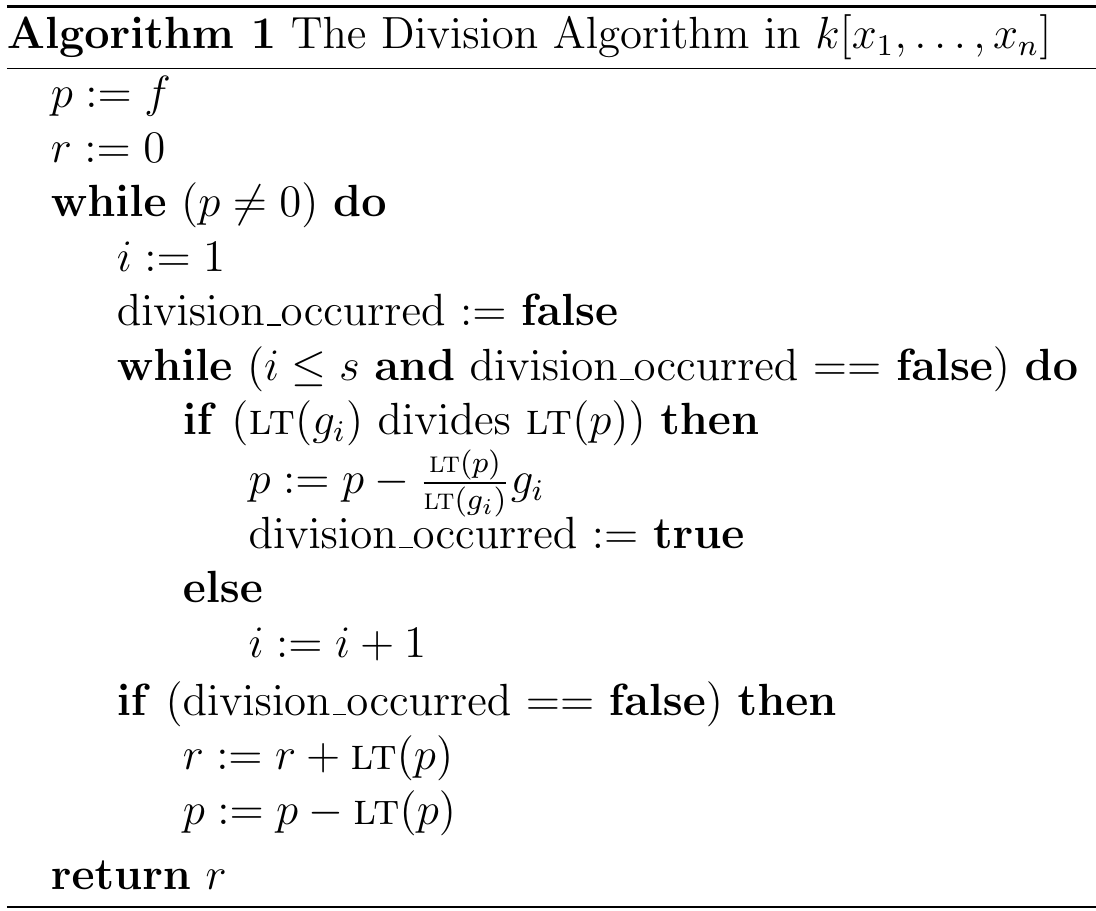
\includegraphics[width=.75\textwidth]{DivisionAlgorithm.png}
\end{frame}

\begin{frame}{Algorithms}
  Given a set $T$, denote the set of finite ordered lists of elements of $T$ as $[T]$. Let $\emptyset \in [T]$ denote the empty list.
\end{frame}

\begin{frame}{Algorithms}
  \[ \scriptstyle \p: [k[\mathbf x]] \times \left( k[\mathbf x] \times k[\mathbf x] \right) \to k[\mathbf x] \times k[\mathbf x] \]
  \[ \scriptstyle \p(G,(p,r)) = \begin{cases}\scriptstyle (p-\LT(p),r+\LT(p)) &\scriptstyle\text{if } G = \emptyset, \\ \scriptstyle (p-\frac{\LT(p)}{\LT(g_1)}g_1,r) &\scriptstyle\text{if } G \ne \emptyset \and \LT(g_1) \mid \LT(p), \\ \scriptstyle \p(G\setminus g_1,(p,r)) &\scriptstyle\text{if } G \ne \emptyset \and \LT(g_1) \nmid \LT(p). \end{cases} \]
  \[ \scriptstyle \psi: [k[\mathbf x]] \times \left( k[\mathbf x] \times k[\mathbf x] \right) \to k[\mathbf x] \]
  \[ \scriptstyle \psi(G,(p,r)) = \begin{cases} \scriptstyle r &\scriptstyle\text{if } p = 0, \\ \scriptstyle \psi(G,\p(G,(p,r))) &\scriptstyle\text{if } p \ne 0. \end{cases} \]
  \[ \scriptstyle \overline f^{G} = \psi(G,(f,0)). \]
\end{frame}

\begin{frame}{Algorithms}
  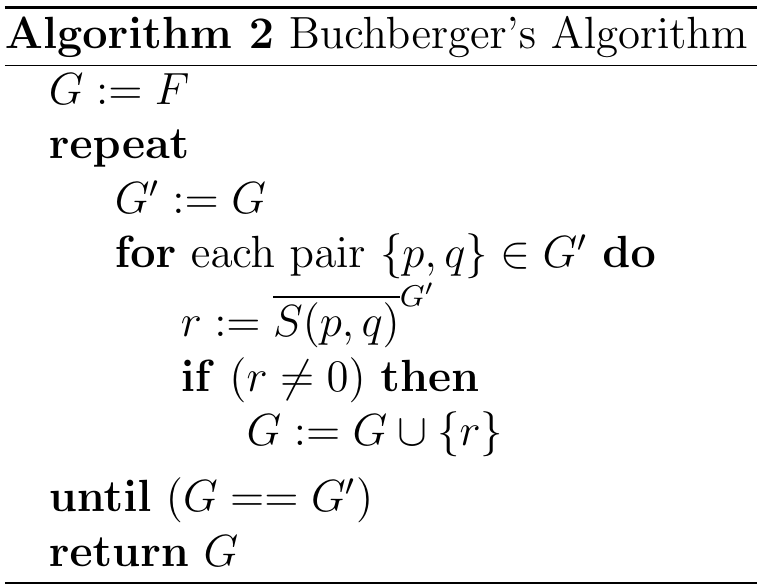
\includegraphics[width=.65\textwidth]{BuchbergersAlgorithm.png}
\end{frame}

\begin{frame}{Algorithms}
  Notation
  \begin{itemize}
    \item<2-> $X + t$
    \item<3-> $X + Y$
    \item<4-> $y \times X$
    \item<5-> $X \times Y$
    \item<6-> For $x = (f,g) \in k[\mathbf x] \times k[\mathbf x]$, $Sx = S(f,g)$.
  \end{itemize}
\end{frame}

\begin{frame}{Algorithms}
  \[ \scriptstyle \p: [k[\mathbf x] \times k[\mathbf x]] \times [k[\mathbf x]] \to [k[\mathbf x]] \]
  \[ \scriptstyle \p(X,G) = \begin{cases} \scriptstyle G &\scriptstyle\text{if } X = \emptyset, \\ \scriptstyle \p(X \setminus x_1,G) &\scriptstyle\text{if } X \ne \emptyset \and \overline{Sx_1}^{G} = 0, \\ \scriptstyle \scriptstyle \p\left(X \setminus x_1 + (\overline{Sx_1}^{G} \times G),G + \overline{Sx_1}^{G}\right) &\scriptstyle\text{if } X \ne \emptyset \and \overline{Sx_1}^{G} \ne 0. \end{cases} \]
  \[ \scriptstyle \gb: [k[\mathbf x]] \to [k[\mathbf x]] \]
  \[ \scriptstyle \gb(F) = \p(F \times F,F) \]
\end{frame}

\begin{frame}{Why?}
  \center {\Large Why should we care?}
\end{frame}

\begin{frame}{End}
  \center {\Large Questions?}
\end{frame}

\end{document}
